\section{Zusammenwirken mehrerer Systeme (Analoge Regelung)}

\subsection{Regelkreis}
\begin{tcolorbox}
\boxtitle{Wichtige Begriffe und Signalbezeichnungen}
\begin{itemize}
  \item \textbf{Führungsgröße:} $w(t)$ (Sollwert)
  \item \textbf{Störgrößen:} $z(t)$ bzw. $z_1(t), z_2(t), z_3(t)$
  \item \textbf{Regelgröße:} $x(t)$ (Istwert)
  \item \textbf{Stellgröße:} $y(t)$ bzw. $u(t)$ (Reglerausgang)
  \item \textbf{Regeldifferenz / Regelabweichung:} $e(t) = w(t) - x(t)$
  \item \textbf{Maximale Überschwingweite:} $h_{\max}$ (maximale Regelabweichung nach erstmaligem Erreichen des Sollwertes)
  \item \textbf{Anregelzeit $t_{\text{an}}$:} Zeit bis zum erstmaligen Erreichen des Sollwertes
  \item \textbf{Ausregelzeit $t_{\text{aus}}$:} Zeit bis zum dauerhaften Verbleib im vorgegebenen Toleranzband (z.\,B. $\pm 2\%$ oder $\pm 5\%$)
\end{itemize}
\end{tcolorbox}

\begin{tcolorbox}
\boxtitle{Anforderungen an den Regelkreis}
\begin{itemize}
  \item \textbf{Stabilität:} Der geschlossene Regelkreis muss stabil sein (auch bei grenzstabilen oder instabilen Strecken).
  \item \textbf{Gutes Führungsverhalten:} Kleines oder kein Überschwingen, schnelle Ausregelung, keine bleibende Regelabweichung.
  \item \textbf{Gutes Störverhalten:} Rasche Dämpfung und Unterdrückung von äußeren Störungen $z(t)$.
\end{itemize}
\end{tcolorbox}

\begin{tcolorbox}
\boxtitle{Grundstruktur des einschleifigen Regelkreises}
\begin{center}
  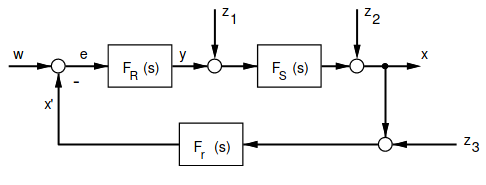
\includegraphics[width=\columnwidth]{images/regelkreis_grundstruktur.png}
\end{center}
Überlagerung der Einflüsse auf die Regelgröße $X(s)$:
\[
X(s) = \frac{F_v}{1 + F_v F_r} W(s) + \frac{1}{1 + F_v F_r} Z_1(s) - \frac{F_v F_r}{1 + F_v F_r} Z_2(s)
\]
Mit $F_0(s) = F_R(s) \cdot F_S(s) \cdot F_r(s)$ (Frequenzgang des offenen Kreises) und $F_r(s) = 1$ (Einheitsrückführung):
\begin{align*}
F_w(s) &= \frac{F_R(s) F_S(s)}{1 + F_0(s)} \quad \text{(Führungsübertragungsfunktion)} \\
F_{z1}(s) &= \frac{1}{1 + F_0(s)} \quad \text{(Störübertragungsfunktion 1)} \\
F_{z2}(s) &= \frac{-F_S(s) F_r(s)}{1 + F_0(s)} \quad \text{(Störübertragungsfunktion 2)}
\end{align*}
\end{tcolorbox}

\subsection{Wurzelortskurven (WOK)-Verfahren}
\begin{tcolorbox}
Aufspaltung der Reglerübertragungsfunktion in Verstärkung $K$ und Reglerdynamik $F_R'(s)$:
\[
F_R(s) = K \cdot F_R'(s) \implies F_0(s) = K \cdot Q \cdot \frac{\prod_{\mu=1}^m (s - s_{N0\mu})}{\prod_{\nu=1}^n (s - s_{P0\nu})}
\]
Pole des geschlossenen Regelkreises erfüllen die charakteristische Gleichung:
\[
1 + F_0(s) = 0 \implies F_0(s) = -1
\]
Aufteilung in Betrags- und Phasenbedingung:
\begin{align*}
\textbf{Betrag:} \quad &\frac{\prod_{\nu=1}^n |s - s_{P0\nu}|}{\prod_{\mu=1}^m |s - s_{N0\mu}|} = |K \cdot Q| \\
\textbf{Phase:} \quad &\sum_{\nu=1}^n \angle(s - s_{P0\nu}) - \sum_{\mu=1}^m \angle(s - s_{N0\mu}) = \pm r \cdot 180^\circ
\end{align*}
wobei $r = 1, 3, 5, \dots$ für $K \cdot Q > 0$ und $r = 0, 2, 4, \dots$ für $K \cdot Q < 0$.
\end{tcolorbox}

\begin{tcolorbox}
\boxtitle{Konstruktionsregeln für die WOK}
\begin{enumerate}
  \item \textbf{Startpunkte:} Die $n$ Äste der WOK beginnen für $K = 0$ in den $n$ Polen $s_{P0\nu}$ des offenen Kreises.
  \item \textbf{Endpunkte:} $m$ Äste enden für $K \to \infty$ in den $m$ Nullstellen $s_{N0\mu}$.
  \item \textbf{Asymptoten:} $n - m$ Äste (Polüberschuss) streben für $K \to \infty$ ins Unendliche.
  \item \textbf{Asymptotengeometrie:}
  \begin{itemize}
    \item Wurzelschwerpunkt (Schnittpunkt auf der reellen Achse):
    \[
    s_w = \frac{\sum_{\nu=1}^n s_{P0\nu} - \sum_{\mu=1}^m s_{N0\mu}}{n - m}
    \]
    \item Asymptotenwinkel mit der positiven reellen Achse:
    \[
    \varphi_k = \frac{(2k - 1) \cdot 180^\circ}{n - m} \quad (k = 1, \dots, n-m \text{ bei } KQ > 0)
    \]
  \end{itemize}
  \item \textbf{Symmetrie:} Die WOK ist spiegelsymmetrisch zur reellen Achse.
  \item \textbf{Reelle Achse:} Ein Punkt auf der reellen Achse gehört zur WOK, wenn rechts von ihm eine \textbf{ungerade} Anzahl reeller Pole und Nullstellen liegt (bei $KQ > 0$).
\end{enumerate}
\textbf{Stabilitätsgrenze:} Schnittpunkte der WOK mit der Imaginärachse liefern $s_{\text{krit}} = j\omega_{\text{krit}}$. Einsetzen in die Betragsbedingung ergibt die kritische Verstärkung $K_{\text{krit}}$.
\end{tcolorbox}

\subsection{Nyquist-Kriterium}
\begin{tcolorbox}
Frequenzgang des offenen Regelkreises: $F_0(j\omega) = F_R(j\omega) F_S(j\omega) F_r(j\omega)$.\\[2pt]
\textbf{Schwingbedingung:}
\[
F_0(j\omega_{\text{krit}}) = -1 = 1 \cdot e^{-j 180^\circ}
\]
Die Schwingbedingung ist erfüllt, wenn die Ortskurve von $F_0(j\omega)$ durch den kritischen Punkt $P_{\text{krit}} = -1 + j0$ verläuft.
\end{tcolorbox}

\begin{tcolorbox}
\boxtitle{Vereinfachtes Nyquist-Kriterium (Linke-Hand-Regel)}
Voraussetzung: Die offene Übertragungsfunktion $F_0(s)$ besitzt \textbf{keine} Pole in der rechten $s$-Halbebene und maximal zwei Pole im Ursprung ($s=0$).\\[3pt]
\textbf{Kriterium:} Der geschlossene Regelkreis ist genau dann \textbf{asymptotisch stabil}, wenn beim Durchlaufen der Ortskurve von $F_0(j\omega)$ in Richtung wachsender Frequenz ($\omega = 0 \to \infty$) der kritische Punkt $P_{\text{krit}} = -1 + j0$ stets \textbf{zur Linken} liegt.
\end{tcolorbox}

\begin{tcolorbox}
\boxtitle{Stabilität im Bode-Diagramm}
Bei minimalphasigen Strecken ist der Regelkreis stabil, wenn die Durchtrittsfrequenz $\omega_{A=1}$ kleiner ist als die Phasenschnittfrequenz $\omega_{\varphi=-180^\circ}$:
\[
\omega_{A=1} < \omega_{\varphi=-180^\circ}
\]
\textbf{Stabilitätsränder:}
\begin{itemize}
  \item \textbf{Phasenrand (Phasenreserve):}
  \[
  \varphi_R = \varphi(\omega_{A=1}) - (-180^\circ) = \varphi(\omega_{A=1}) + 180^\circ
  \]
  \item \textbf{Amplitudenrand (Verstärkungsreserve):}
  \[
  A_R = \frac{1}{|F_0(j\omega_{\varphi=-180^\circ})|} \quad \text{bzw.} \quad A_{R,\text{dB}} = -20 \lg |F_0(j\omega_{\varphi=-180^\circ})|
  \]
\end{itemize}
\end{tcolorbox}

\begin{center}
  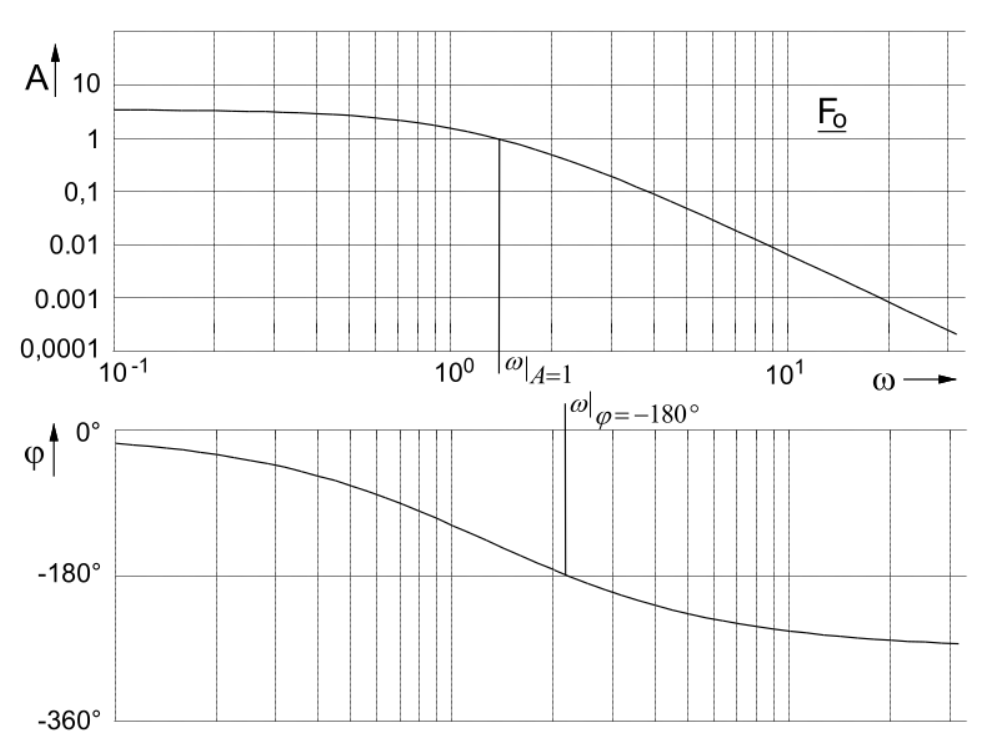
\includegraphics[width=0.9\columnwidth]{images/bode_raender.png}
\end{center}

\begin{tcolorbox}
\boxtitle{Allgemeines Nyquist-Kriterium}
Gilt auch für instabile offene Systeme. Der geschlossene Kreis ist stabil, wenn der Fahrstrahl von $P_{\text{krit}} = -1+j0$ zur Ortskurve $F_0(j\omega)$ für $\omega = +0 \to +\infty$ eine Winkeländerung von
\[
\Delta \varphi_{\text{soll}} = n_r \cdot 180^\circ + n_a \cdot 90^\circ
\]
im mathematisch positiven Sinn (gegen den Uhrzeigersinn) erfährt.
\begin{itemize}
  \item $n_r$: Anzahl der Pole des offenen Kreises in der rechten $s$-Halbebene.
  \item $n_a$: Anzahl der Pole auf der imaginären Achse (ohne Ursprung).
\end{itemize}
\end{tcolorbox}

\subsection{Reglerauslegung im Bode-Diagramm}
\begin{tcolorbox}
\begin{itemize}
  \item \textbf{Kleine bleibende Regeldifferenz:} $A(\omega) \gg 1$ bei tiefen Frequenzen ($\omega \ll \omega_{A=1}$).
  \item \textbf{Stabilität:} $\varphi(\omega_{A=1}) > -180^\circ \iff \varphi_R > 0$.
  \item \textbf{Empfohlene Phasenränder:}
  \begin{itemize}
    \item Befriedigendes Störverhalten: $\varphi_R \ge 30^\circ$
    \item Gutes Führungsverhalten (überschwingungsarm): $\varphi_R \approx 60^\circ$
    \item Überschwingungsfrei (aperiodisch): $\varphi_R \ge 80^\circ$
  \end{itemize}
  \item \textbf{Unterdrückung von hochfrequenten Störungen:} $A(\omega) \ll 1$ für $\omega \gg \omega_{A=1}$.
\end{itemize}
\end{tcolorbox}

\subsection{Einstellregeln}

\subsubsection{Ziegler/Nichols (Schwingungsmethode)}
\begin{tcolorbox}
Regelkreis mit reinem P-Regler betreiben. Verstärkung $K_P$ erhöhen, bis Dauerschwingung an der Stabilitätsgrenze auftritt. $K_{P,\text{krit}}$ und Periodendauer $T_{\text{krit}}$ notieren:
\begin{center}
\small
\begin{tabular}{l l l l}
\toprule
\textbf{Reglertyp} & $K_P$ & $T_N$ & $T_V$ \\
\midrule
\textbf{P} & $0{,}50 \cdot K_{P,\text{krit}}$ & -- & -- \\
\textbf{PI} & $0{,}45 \cdot K_{P,\text{krit}}$ & $0{,}85 \cdot T_{\text{krit}}$ & -- \\
\textbf{PD} & $0{,}80 \cdot K_{P,\text{krit}}$ & -- & $0{,}12 \cdot T_{\text{krit}}$ \\
\textbf{PID} & $0{,}60 \cdot K_{P,\text{krit}}$ & $0{,}50 \cdot T_{\text{krit}}$ & $0{,}12 \cdot T_{\text{krit}}$ \\
\bottomrule
\end{tabular}
\end{center}
\textbf{Nachteil:} System muss an die Stabilitätsgrenze gefahren werden (bei vielen realen Anlagen wegen Zerstörungsgefahr unzulässig).
\end{tcolorbox}

\subsubsection{Betragsoptimum (BO)}
\begin{tcolorbox}
Anwendbar für Strecken mit $PT_n$-Verhalten mit einer dominierenden (großen) Zeitkonstante $T_1 = T_d$ und mehreren kleinen Zeitkonstanten ($T_2, T_3, \dots$):
\[
T_1 = T_d \gg T_2, T_3, \dots, T_n, \quad T_\Sigma = \sum_{i=2}^n T_i, \quad K_S = \prod_{i=1}^n K_i
\]
Einstellung des PI-Reglers $F_{PI}(s) = K_R \left(1 + \frac{1}{T_N s}\right)$:
\[
T_N = T_d, \qquad K_R = \frac{T_d}{2 \cdot K_S \cdot T_\Sigma}
\]
\end{tcolorbox}

\subsubsection{Symmetrisches Optimum (SO)}
\begin{tcolorbox}
Anwendbar für Strecken mit $IT_n$-Verhalten (integrierendes Verhalten mit reellen Verzögerungen $T_1, T_2, \dots$):
\[
T_\Sigma = \sum_{i=1}^n T_i, \qquad K_S = \prod_{i=1}^n K_i
\]
Einstellung des PI-Reglers:
\[
T_N = 4 \cdot T_\Sigma, \qquad K_R = \frac{1}{2 \cdot K_S \cdot T_\Sigma} \quad (\varphi_R \approx 40^\circ)
\]
\end{tcolorbox}

\subsection{Maßnahmen zur Verbesserung des Regelverhaltens}

\begin{tcolorbox}
\boxtitle{Störgrößenaufschaltung}
\begin{center}
  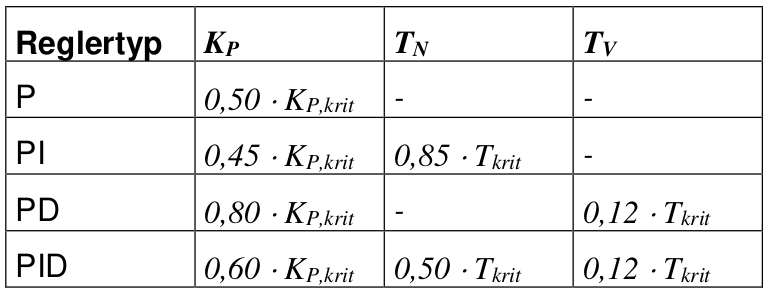
\includegraphics[width=\columnwidth]{images/stoergroessenaufschaltung.png}
\end{center}
Voraussetzung: Störgröße $z$ ist messbar und ihr Angriffsort bekannt. Das Störsignal wird über $F_{Sz}(s)$ direkt kompensiert, bevor es die Regelgröße auslenkt. Sehr schnelle Ausregelung ohne Stabilitätsverlust.
\end{tcolorbox}

\begin{tcolorbox}
\boxtitle{Vorsteuerung}
\begin{center}
  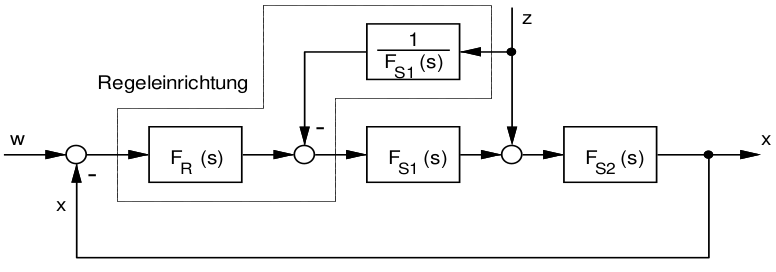
\includegraphics[width=\columnwidth]{images/vorsteuerung.png}
\end{center}
Wird eingesetzt, wenn kein optimaler Kompromiss zwischen Führungs- und Störverhalten möglich ist. Der Hauptregler wird auf gutes Störverhalten ausgelegt; der Vorsteuerfilter $F_{Rv}(s)$ beschleunigt das Folgen von $w(t)$.
\end{tcolorbox}

\begin{tcolorbox}
\boxtitle{Kaskadenregelung}
\begin{center}
  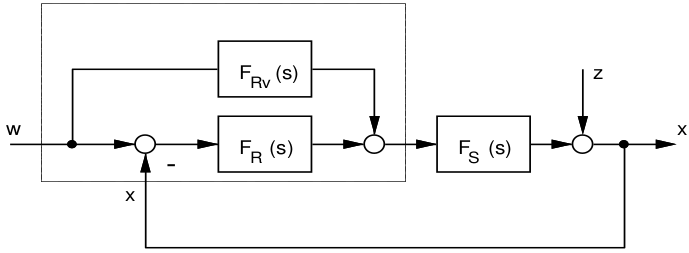
\includegraphics[width=\columnwidth]{images/kaskadenregelung.png}
\end{center}
Ineinandergeschachtelte Kreise. Der innere Hilfskreis ist deutlich schneller und regelt innere Störungen sofort aus. Inbetriebnahme erfolgt von innen nach außen.
\end{tcolorbox}

\begin{tcolorbox}
\boxtitle{Führungsgrößenfilter}
\begin{center}
  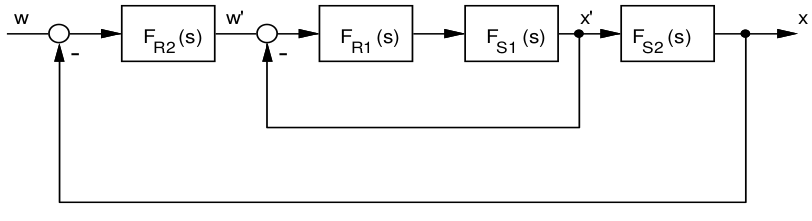
\includegraphics[width=0.9\columnwidth]{images/fuehrungsgroessenfilter.png}
\end{center}
Dominiert eine Nullstelle den geschlossenen Kreis, kommt es zu hohem Überschwingen. Ein vorgeschaltetes $PT_1$-Filter kompensiert diese Nullstelle exakt.
\end{tcolorbox}

\begin{tcolorbox}
\boxtitle{Anti-Windup (Grundprinzip)}
Bei Stellgrößenbegrenzung und I-Anteil läuft der Integrator unbegrenzt weiter (Windup), was zu extremem Überschwingen führt. Lösung: Begrenzung oder Anhalten des I-Anteils, sobald die Stellgrenze erreicht ist.
\end{tcolorbox}
